\graphicspath{{Chapter2/Figs/}}

\chapter{Multi-Omics Factor Analysis (MOFA), a Bayesian model for integration of multi-omics data}

The work described in this chapter results from a collaboration with Wolfgang Huber's group at the EMBL (Heidelberg, Germany). It has been peer-reviewed and published in \cite{Argelaguet2018}.\\
The method was conceived by Florian Buettner, Oliver Stegle and me. I performed most of the mathematical derivations and implementation, but with significant contributions from Damien Arnol and Britta Velten. The CLL data application was led by Britta Velten whereas the single-cell application was lead by me, but with joint contributions in either cases. Florian Buettner, Wolfgang Huber and Oliver Stegle supervised the project.\\
The article was jointly written by Britta Velten and me, with contributions from all authors.

\section{Theoretical foundations}

\subsection{Mathematical notation} \label{section:mathematical_notation}

\begin{itemize}[noitemsep]
	\item[--] Matrices are denoted with bold capital letters: $\bfW$
	\item[--] Vectors are denoted with bold non-capital letters: $\bfw$. If the vector comes from a matrix, we will use a single index to indicate the row that it comes from. If two indices are used, the first one corresponds to the row and the second one to the column. The symbol '$:$' denotes the entire row/column. For instance, $\bfw_{i}$ refers to the $i$th row from the $\bfW$ matrix, whereas $\bfw_{:,j}$ refers to the $j$th column.
	\item[--] Scalars are denoted with non-bold and non-capital letters: $w$. If the scalar comes from a 1-dimensional array (a vector), a single subscript will indicate its position in the vector. If the scalar comes from a 2-dimensional array, two indices will be shown at the bottom: the first one corresponding to the row and the second one to the column. For instance, $w_{i,j}$ refers to the value from the $i$th row and the $j$th column of the matrix $\bfW$, and $w_i$ to the $i$th value of the vector $\bfw$. In some cases, higher dimensional arrays (tensors) are used, and the use of multiple indices follows the same rationality.
	\item[--] $\boldzero_k$ is a zero vector of length $K$.
	\item[--] $\I_k$ is the identity matrix with rank $K$.
	\item[--] $\E_q[x]$ denotes the expectation of $x$ under the distribution $q$. When the expectations are taken with respect to the same distribution many times, we will avoid cluttered notation and we will instead use $\la x \ra$.
	\item[--] $\Ndist{x}{\mu,\sigma}$: $x$ follows a univariate normal distribution with mean $\mu$ and variance $\sigma$.
	\item[--] $\Gdist{x}{a,b}$: $x$ follows a gamma distribution with shape and rate parameters $a$ and $b$.
	\item[--] $\Bdist{x}{a, b}$: $x$ follows a beta distribution with shape and rate parameters $a$ and $b$.
	\item[--] $\text{Ber}(x, \theta)$: $x$ follows a Bernoulli distribution with parameter $\theta$.
	\item[--] $\mathds{1}_0$: Dirac delta function centered at 0.
	\item[--] $Tr(\bfX)$: Trace of the matrix \bfX
\end{itemize}

\subsection{Graphical notations for probabilistic models}

Probabilistic models can be represented in a diagrammatic format (i.e. a graph or a network) that offers a compact visual representation of complicated systems of probability distributions \cite{Bishop2006}. In a graphical model the relationship between the nodes becomes more explicit, namely their conditional independence properties which allow the joint distribution over all variables to be factorised into a series of simpler products involving subsets of variables \cite{Bishop2006}. The basic unit of a network is the node, which represents the different types of variables, including observed variables, unobserved probabilistic variables and unobserved parameters. The nodes are connected by unidirectional edges (arrows) which capture the conditional independence relationship between the variables.

For this thesis we adapted the graphical notations from~\cite{Dietz2010-technical-report-graphs}:

\begin{center}
  \begin{tabular}{m{8cm} m{2cm}}
    Observed variables & \tikz{\node[obs](){$Y$}} \\
    Unobserved probabilistic variables & \tikz{\node[latent](){$\theta$}} \\
    Unobserved parameters & \tikz{\node[latent,double, double distance=1pt](){$\theta$}} \\
    Repetition of node $\theta_n$ for $n\in\llbracket 1;N \rrbracket$ & \tikz{\node[latent](theta){$\theta_n$}; \plate[] {plateN} {(theta)} {$N$};} \\
    Conditional dependency between nodes: $p(Y,\theta) = p(Y|\theta)p(\theta)$ & \tikz{%
            \node[latent]   (theta) {$\theta$};
            \node[obs, xshift=1.5cm] (Y) {$Y$};
            \edge{theta}{Y}}
  \end{tabular}
\end{center}
% For simplicity, fixed hyperparameters are not represented on the graphical model. Unobserved parameters are only represented when optimised together with the unobserved probabilistic variables.



\subsection{Probabilistic modelling} \label{section:probabilistic_modelling}

A scientific model is a simple theoretical representation of a complex natural phenomenon to allow the systematic study of its behaviour. The general idea is that if a model is able to explain some observations, it might be capturing its true underlying laws and can therefore be used to make future predictions.
In particular, statistical models are a powerful abstraction of nature. They consist on a set of observed variables and a set of (hidden) parameters. The procedure of fitting the parameters using a set of observations is called inference or learning.

One of the major challenges of inference when dealing with real data sets is the distinction between signal and noise. An ideal model should learn only the information relevant to gain explanatory power while disregarding the noise. However, this is a non-trivial task in most practical situations. Very complex models will tend to overfit the training data, capturing large amounts of noise and consequently leading to a bad generalisation performance to independent data sets. On the other hand, simplistic models will fit the data poorly, leading to poor explanatory power.

The ideas above can be formalised using the framework of probability and statistics.


\subsubsection{Maximum likelihood inference} \label{section:maximum_likelihood}

A common approach is to define a statistical model of the data $\bfY$ with a set of parameters $\btheta$ that define a probability distribution $p(\bfY|\btheta)$, called the likelihood function. A simple approach to fit a model is to estimate the parameters $\hat{\btheta}$ that maximise the likelihood:
\[
	\hat{\btheta} = \argmax_{\btheta} p(\bfY|\btheta)
\]
This process is called maximum likelihood learning\cite{Stigler2008,Bishop,Murphy}. However, in this setting there is no penalisation for model complexity, making maximum likelihood solutions prone to overfit in cases where the data is relatively sparse. Generalisations that account for model complexity have been proposed and include regularising terms that shrink parameters to small values. However, these are often particular cases of the more general framework of Bayesian statistics \cite{Hastie,Bishop,Murphy}.

\subsubsection{Bayesian inference}  \label{section:bayesian_inference}
In the Bayesian framework, the parameters themselves are treated as random unobserved variables and we aim to obtain probability distributions for $\btheta$, rather than a single point estimate. To do so, prior beliefs are introduced into the model by specifying a prior probability distribution $p(\btheta)$. Then, using Bayes' theorem \cite{Bayes1763}, the prior hypothesis is updated based on the observed data $\bfY$ by means of the likelihood $p(\bfY|\btheta)$ function, which yields a posterior distribution over the parameters:
\[
	p(\btheta|\bfY) = \frac{p(\bfY|\btheta) p(\btheta)}{p(\bfY)}
\]
where $p(\bfY)$ is a constant term called the marginal likelihood, or model evidence \cite{Bishop,Murphy}.\\
The choice of the prior distribution is a key part of Bayesian inference and captures beliefs about the distribution of a variable before the data is taken into account. With asymptotically large sample sizes, the choice of prior has negligible effects on the posterior estimates, but it becomes critical with sparse data \cite{Bishop,Murphy,Gelman2013}.

There are two common considerations when defining the prior distributions. The first relates to the incorporation of subjective information, or predefined assumptions, into the model. For example, one could adapt the prior distribution to match the results from previous experiments (i.e. an informative prior). Alternatively, if no information is available one could set set uninformative priors by following maximum entropy principles \cite{Jaynes1968}.

The second strategy is based on convenient mathematical properties to make inference tractable. If the likelihood and the prior distributions do not belong to the same family of probability distributions (they are not conjugate) then inference becomes more problematic \cite{Raiffa1961,Bishop,Murphy,Gelman2013}. The existence of conjugate priors is one of the major reasons that justify the widespread use of exponential family distributions in Bayesian models \cite{Gelman2013}. An example is the Automatic Relevance Determination prior discussed in \Cref{section:ard}.

Again, the milestone of Bayesian inference is that an entire posterior probability distribution is obtained for each unobserved variable. This has the clear advantage of naturally handling uncertainity in the estimation of parameters. For instance, when making predictions, a fully Bayesian approach attempts to integrate over all the possible values of all unobserved varaibles, effectively propagating uncertainity across multiple layers of the model. Nevertheless, this calculation is sometimes intractable and one has to resort to point estimates \cite{Bishop,Murphy,Gelman2013}. The simplest approximation to the posterior distribution is to use its mode, which leads to the maximum a posteriori (MAP) estimate:
\[
	\hat{\btheta} = \argmax_{\btheta} p(\btheta) p(\bfY|\btheta) 
\]
This is similar to the maximum likelihood objective function, but with the addition of a term $p(\btheta)$. When the prior dsitribution is chosen smartly, this term penalises for model complexity. Therefore, in contrast to standard (non-penalised) maximum likelihood inference, Bayesian approaches naturally handle the problem of model complexity and overfitting\cite{Bishop,Murphy,Gelman2013}. At the limit of infinite observations, the influence of the prior to the posterior is negligible and the MAP estimate converges towards the Maximum likelihood estimate, hence providing a rational link between the two inference frameworks.

\subsubsection{Deterministic approaches for Bayesian inference} \label{section:deterministic_bayesian_inference}
The central task in Bayesian inference is the direct evaluation of the posterior distributions and/or the computation of expectations with respect to the posterior distributions. In sufficiently complex models, closed-form solutions are not available and one has to resort to approximation schemes, which broadly fall into two classes: stochastic or deterministic \cite{Gelman2013,Blei2016}. 

Stochastic approaches hinge on the generation of samples from the posterior distribution via a Markov Chain Monte Carlo (MCMC) framework. Such techniques have the appealing property of generating exact results at the asymptotic limit of infinite computational resources. However, in practice, sampling approaches are computationally demanding and suffer from limited scalability to large data sets \cite{Blei2016}. \\
In contrast, deterministic approaches are based on analytical approximations to the posterior distribution, which often lead to biased results. Yet, given the appropriate settings, these approaches are potentially much faster and scalable to large applications \cite{Bishop,Murphy,Blei2016}.

\subsubsection{Laplace approximation} \label{section:laplace_approximation}
The Laplace approximation is probably the simplest of the deterministic tecniques, where the aim is to construct a Gaussian approximation around the mode of the true posterior distribution using a second-order Taylor expansion \cite{Bishop,Murphy}.\\
Suppose $\bfX$ contains all unobserved variables. The true posterior distribution can be written as:
\[
p(\bfX) = \frac{f(\bfX)}{Z}
\]
where $f(\bfX)$ is a function that depends on the unobserved variables and $Z$ is an unknown normalisation constant to ensure that $\int p(\bfX) d\bfX = 1$.

The second-order Taylor expansion of $\log f(\bfX)$ centered around its (known) mode $\hat{\bfX}$ is: 
\[
	\log f(\bfX) \approx \log f(\hat{\bfX}) - \frac{1}{2} (\bfX-\hat{\bfX})^T \bfA (\bfX-\hat{\bfX})
\]
where $\bfA = \nabla^2 \log f(\hat{\bfX})$ is the Hessian matrix of $\log f(\bfX)$ evaluated at $\hat{\bfX}$.\\
Notice three things. First, the first-order term of the Taylor expansion is zero because $\hat{\bfX}$ is a stationary point. Second, the $\log$ function is monotonically increasing and therefore a maximum of $\log f(\bfX)$ is also a maximum of $f(\bfX)$. Third, the mode of the posterior $p(\bfX)$ must be known, which requires the use of (complex) optimisation algorithms.\\
Taking the exponential in both sides:
\[
	f(\bfX) \approx f(\hat{\bfX}) \exp\{ -\frac{1}{2} (\bfX-\hat{\bfX})^T \bfA (\bfX-\hat{\bfX}) \}
\]
which leads to the following multivariate Gaussian distribution approximation $q(\bfX) = \Ndist{\bfX}{\hat{\bfX},\bfA}$:
\[
	q(\bfX) = \frac{\mid A \mid^{1/2}}{(2\pi^{d/2})} \exp\{ -\frac{1}{2} (\bfX-\hat{\bfX})^T \bfA (\bfX-\hat{\bfX}) \}
\]
where $d$ is the number of unobserved variables. \\
Despite its simplicity, the Laplace approximation is a useful strategy that has been successfully applied in practice. Nonetheless, this approximation has notable caveats: first, is limited by its own local definition, ignoring all the density beyond the mode of the posterior. Second, it does not apply to discrete variables. Third, the inversion of the Hessian is very expensive in high-dimensional settings.
	% More sophisticated generalisations of the Laplace approximation have also been proposed \cite{Rue2009}
	% To-do: check where does the inverse appear

\subsubsection{Variational inference}  \label{section:variational_inference}

Variational inference is a deterministic family of methods that have been receiving widespread attention due to a positive balance between accuracy, speed, and ease of use \cite{Blei2016, Zhang2017}. The core framework is derived below.

In variational inference the true (but intractable) posterior distribution $p(\bfX|\bfY)$ is approximated by a simpler (variational) distribution $q(\bfX|\bTheta)$ where $\bTheta$ are the corresponding parameters. The parameters, which we will omit from the notation, need to be tuned to obtain the closest approximation to the true posterior.\\
The distance between the true distribution and the variational distribution is calculated using the KL divergence:
\[
\KL(q(\bfX)||p(\bfX|\bfY)) = - \int_z q(\bfX) \log \frac{p(\bfX|\bfY)}{q(\bfX)}
\]
Note that the KL divergence is not a proper distance metric, as it is not symmetric. In fact, using the reverse KL divergence $\KL(q(\bfX)||p(\bfX|\bfY))$ defines a different inference framework called expectation propagation \cite{Minka2001}.

If we allow any possible choice of $q(\bfX)$, then the minimum of this function occurs when $q(\bfX)$ equals the true posterior distribution $p(\bfX|\bfY)$. Nevertheless, since the true posterior is intractable to compute, this does not lead to any simplification of the problem. Instead, it is necessary to consider a restricted family of distributions $q(\bfX)$ that are tractable to compute and subsequently seek the member of this family for which the KL divergence is minimised.

Doing some calculus it can be shown (see \cite{Bishop,Murphy}) that the KL divergence $\KL(q(\bfX)||p(\bfX|\bfY))$ is the difference between the log of the marginal probability of the observations $\log(\bfY)$ and a term $\Lagr(\bfX)$ that is typically called the Evidence Lower Bound (ELBO):
\[
	\KL(q(\bfX)||p(\bfX|\bfY)) = \log(\bfX) - \Lagr(\bfX)
\]
Hence, minimising the KL divergence is equivalent to maximising $\Lagr(\bfX)$ \Cref{fig:ELBO}:
\begin{align} \label{eq_elbo1} \begin{split}
	\Lagr(\bfX) &= \int q(\bfX) \Big( \log \frac{p(\bfX|\bfY)}{q(\bfX)} + \log p(\bfY) \Big) d\bfX \\
	%&= \int \Big( q(\bfX) \log \frac{p(\bfX|\bfY)}{q(\bfX)} + q(\bfX)\log p(\bfY) \Big) d\bfX\\
	%&= \E_q [\log p(\bfX|\bfY)] - \E_q [\log q(\bfX)] + \E_q [\log p(\bfY)] \\
	&= \E_q [\log p(\bfX,\bfY)] - \E_q [\log q(\bfX)]
\end{split} \end{align}
The first term is the expectation of the log joint probability distribution with respect to the variational distribution. The second term is the entropy of the variational distribution.
Importantly, given a simple parametric form of $q(\bfX)$, each of the terms in \Cref{eq_elbo1} can be computed in closed form.\\
In some occasions (see section X), we will use the following form for the ELBO:
\begin{equation} \label{eq_elbo2}
	\Lagr(\bfX) = \E_q [\log p(\bfY|\bfX)] + (\E_q [\log p(\bfX)] - \E_q [\log q(\bfX)])
\end{equation}
where the first term is the expectation of the log likelihood and the second term is the difference in the expectations of the $p$ and $q$ distributions of each hidden variable.

In conclusion, variational learning involves minimising the KL divergence between $q(\bfX)$ and $p(\bfX|\bfY)$ by instead maximising $\Lagr(\bfX)$ with respect to the distribution $q(\bfX)$. The following image summarises the general picture of variational learning:

\begin{figure}[H]
	\centering
	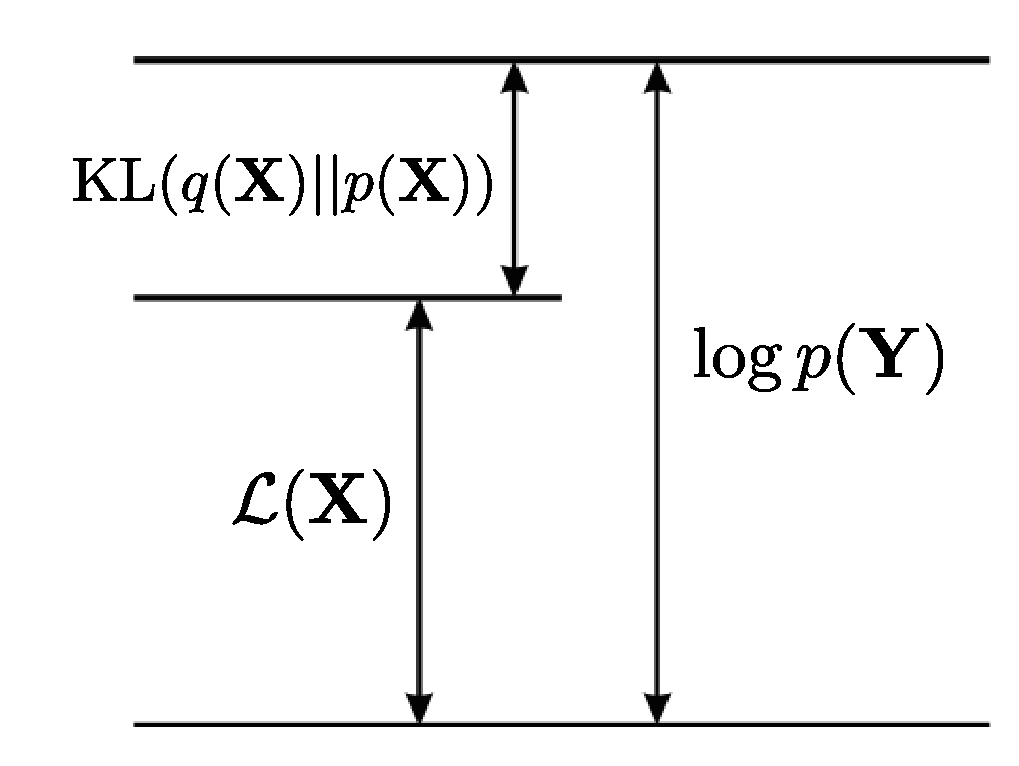
\includegraphics[width=0.35\linewidth]{lower_bound}
	\caption{The quantity $\Lagr(\bfX)$ provides a lower bound on the true log marginal likelihood $\log p(\bfY)$, with the difference being given by the Kullback-Leibler divergence $\KL(q||p)$ between the variational distribution $q(\bfX)$ and the true posterior $p(\bfX|\bfY)$}
	\label{fig:ELBO}
\end{figure}

There are several approaches to define $q(\bfX)$, the two most commonly used are called (unparametric) mean-field and (parametric) fixed-form \cite{Zhang2017,Blei2016}.

\subsubsection{Mean-field variational inference}  \label{section:mean_field}

The most common type of variational Bayes, known as the mean-field approach, assumes that the variational distribution factorises over M disjoint groups of unobserved variables\cite{Saul1996}:
\begin{equation} \label{eq:mean_field}
	q(\bfX) = \prod_{i=1}^{M} q(\bfx_i)
\end{equation}
where typically all unobserved variables are assumed to be independent. Importantly, notice that no parametric assumptions were placed regarding the nature of $q(\bfx_i)$.

Evidently, in sufficiently complex models where the unobserved variables have dependencies this family of distributions do not contain the true posterior (\Cref{fig:mean_field}). Yet, this is a key assumption to obtain an analytical inference scheme that yields surprisingly accurate results \cite{Blei2006,Faes2011,Braun2007}.

\begin{figure}[H]
	\centering
	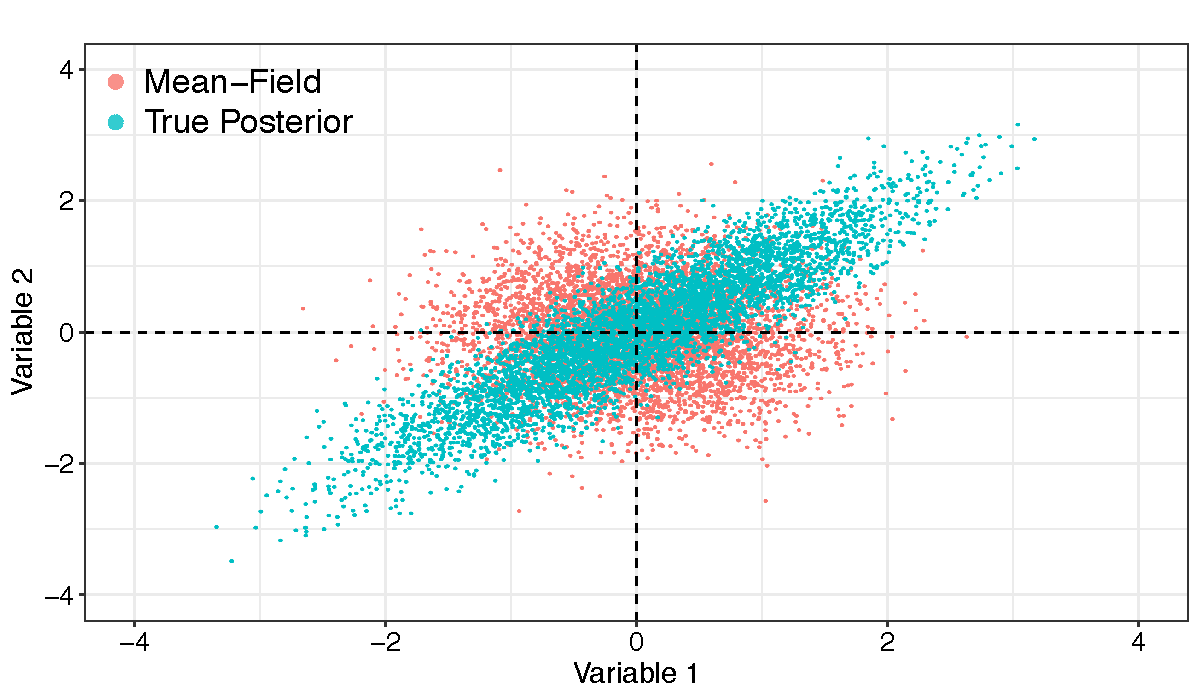
\includegraphics[width=0.7\linewidth]{mean_field}
	\caption{Illustrative example of sampling from a true posterior distribution (blue) versus a fitted mean-field varaitional distribution (red) in a model with two (correlated) unobserved variables. The mean-field approximation wrongly assumes that the unobserved variables are independent.}
	\label{fig:mean_field}
\end{figure}

Using calculus of variations (derivations can be found in \cite{Bishop,Murphy}), it follows that the optimal distribution $q(\bfX)$ that maximises the lower bound $\Lagr(\bfX)$ is
\begin{equation} \label{eq:optimal}
	\log \hat{q}_i(\bfx_i) = \E_{-i} [\log p(\bfY,\bfX)] + \mathrm{const}
\end{equation}
where $\E_{-i}$ denotes an expectation with respect to the $q$ distributions over all variables $\bfx_j$ except for $\bfx_i$.\\
The additive constant is set by normalising the distribution $\hat{q}_i(\bfz_i)$:
\[
	\hat{q}(\bfx_i) = \frac{\exp(\E_{-i}[\log p(\bfY,\bfX)])}{\int \exp(\E_{-i}[\log p(\bfY,\bfX)]) d\bfX}
\]
While the form of $\hat{q}(\bfx_i)$ is not restricted to a specific parametric form, it can be shown that when using conjugate priors, the distributions $\hat{q}_i(\bfx_i)$ have the same functional form as the priors $\hat{p}(\bfx_i)$. 
%An example is shown in Appendix X, but a detailed mathematical treatment with derivations of multiple examples can be found in \cite{Bishop,Murphy,Zhao2009}.


\subsubsection{Fixed-form variational inference}  \label{section:fixed_form}

An alternative and straightforward choice is to directly define a parametric form for the distribution $q(\bfX)$ with some parameters $\bTheta$. Once the choice of $q(\bfX)$ is made, the parameters $\bTheta$ are optimised to minimise $\KL(q(\bfX)||p(\bfX|\bfY))$ (the variational problem):
\begin{align}
	\hat{\bTheta} &= \argmin_{\bTheta} \KL(q(\bfX)||p(\bfX|\bfY)) \\
	&= \E[\log(q(\bfX)) - \log(p(\bfX,\bfY))]
\end{align}
Numerically optimising this function requires the evaluation of expectations with respect to $q(\bfX)$. In closed form, this is only feasable for a limited group of variational distributions. Alternatively, one can attempt Monte Carlo approximations, but in practice this turns to be slow and leads to high-variance estimates \cite{Braun2007,Ranganath2014,Braun2007}.

Typically, one would choose this distribution to factorise over parameters and to be of the same (exponential) family as the prior $p(\bfX)$. In such case there is a closed form coordinate-ascent scheme available, and it turns out that the fixed-form formulation is equivalent to the (non-parametric) mean-field derivation when using conjugate priors.\\
Unfortunately, for generic models with arbitrary families of distributions, no closed-form variational distributions exist \cite{Zhang2017,Blei2016}. 

However, while the parametric assumption certainly limits the flexibility of variational distributions, the advantage of this formulation is that it unveils the possibility to use fast gradient-based methods for the inference procedure \cite{Hoffman2012,Ranganath2014}.

%\paragraph{Black box variational inference}

\subsubsection{Expectation Propagation}  \label{section:expectation_propagation}

Expectation Propagation (EP) is another deterministic strategy with a similar philosophy as the Variational approach. It is also based on minimising the KL divergence between a variational distribution $q(\bfX)$ and the true posterior $p(\bfX|\bfY)$, but while variational inference minimises $KL(p||q)$, EP maximises the reverse KL-divergence $KL(q||p)$.

Interestingly, this simple difference leads to an inference scheme with stringkly different properties. This can be understood by inspecting the differences between the two KL divergence formulas:

Variational inference:
\begin{equation} \label{eq:kl_vb}
	\KL(q(\bfX)||p(\bfX|\bfY)) = - \int_z q(\bfX) \log \frac{p(\bfX|\bfY)}{q(\bfX)}
\end{equation}
Expectation propagation:
\begin{equation} \label{eq:kl_ep}
	\KL(p(\bfX|\bfY)||q(\bfX)) = - \int_z p(\bfX|\bfY) \log \frac{q(\bfX)}{p(\bfX|\bfY)}
\end{equation}
In regions of $\bfX$ where the true posterior density $p(\bfX|\bfY)$ is small, setting a large density for $q(\bfX)$ has a much stronger penalisation in \Cref{eq:kl_ep} than in \Cref{eq:kl_vb}, because of the true posterior density being on the denominator. Hence, EP tends to avoid areas where the density $p(\bfX|\bfY)$ is very low, even if it does not correspond to areas of very high-density in $p(\bfX|\bfY)$. In contrast, in \Cref{eq:kl_vb} there is a strong penalty for having low-density $q(\bfX)$ values.\\
As discussed in \cite{Bishop}, the practical consequences of this duality can be observed when the posterior is multi-modal, as in any sufficiently complex model. In VI, $q(\bfX)$ converges towards areas of high-density in $p(\bfX|\bfY)$, namely local optima. In contrast, EP tends to capture as much non-zero density regions from $p(\bfX|\bfY)$ as possible, thereby averaging across all optima. In the context of doing predictions, the VI solution is much more desirable than the EP solution, as the average of two good parameter values is not necessarily a good parameter itself.\\
A detailed mathematical treatment of EP, including derivations for specific examples, can be found in \cite{Bishop,Murphy,Minka2001}

\begin{figure}[H]
	\centering
	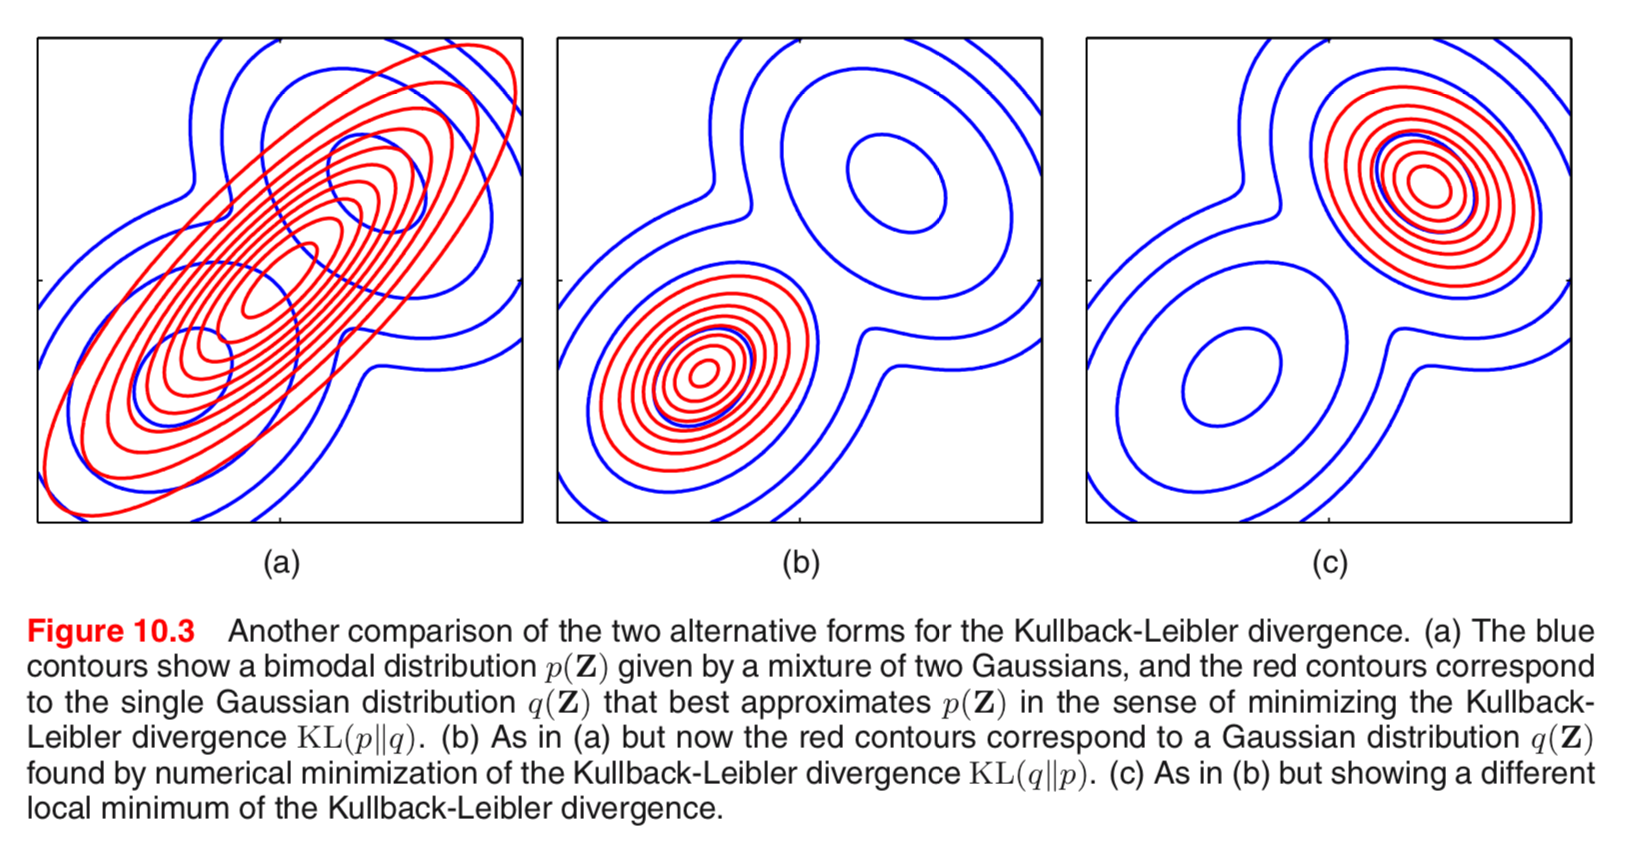
\includegraphics[width=1.0\linewidth]{VB_vs_EP}
	\caption{Illustrative comparison of Variational inference and Expectation Propagation. Shown is the (a) Density and (b) Variance of the true posterior distribution $p(\bfX|\bfY)$ (grey), the variational distribution (orange) and the expectation propagation distribution (green).}
	\label{}
\end{figure}

Following the rationale above, it is easy to predict that variational inference tends to be underestimate the variance of the posterior density. Yet, empirical research have shown that this is acceptable, provided that a good model selection is performed \cite{Blei2006}.


\subsubsection{Conclusions}

In this section we have introduced Bayesian modelling and variational inference methods, which will be used later in this chapter.\\
More generally, variational inference is growing in popularity for the analysis of big data sets and it has been applied to a myriad of different problems, including genome-wide association studies \cite{Carbonetto2012}, population genetics, \cite{Raj2014}, network analysis \cite{Sanguinetti2006} and natural language processing \cite{Blei2003}.

Yet, despite its increasing success, there is significant room for improvement. First and foremost, the theoretical guarantees of variational inference are not as developed as in sampling-based MCMC schemes\cite{Blei2016,Zhang2017,Nakajima2007}. As an example, the mean-field setting makes strong independence assumptions about the parameters.  Although it tends to besurprisingly effective, it is not clear in which applications the dependencies between the parameters are important enough than the mean-field approximation could potentially break.\\
More generally, an open research problem is understanding what are the statistical properties of the variational posterior with respect to the exact posterior \cite{Blei2016,Zhang2017}.

As we shall demonstrate later, alternative strategies have been considered to allow some dependencies between the variables, resulting in \textit{structured} mean-field approximations\cite{Hoffman2014,Titsias2011}. However, they often lead to very complex (if not intractable) inference frameworks. 

Finally, another area of extensive research is how to extend the applicability of VI to non-conjugate models. As discussed in \Cref{section:deterministic_bayesian_inference}, the ELBO of non-conjugate models contains intractable integrals, and setting up an inference scheme requires the use of either stochastic Monte Carlo approximations or deterministic approximations that introduce additional lower bounds \cite{Zhang2017,Seeger2012,Khan2017}. In this thesis we follow this rationale to derive an inference framework for a model with non-gaussian likelihoods.



\subsection{Latent variable models for genomics}

With the exponential growth in the use of high-throughput genomics, biological data sets are increasingly high dimensional, both in terms of samples and features. A key principle of biological data sets is that variation between the features results from differences in underlying, often unobserved, processes. Such processes, whether driven by biological or technical effects, are manifested by coordinated changes in multiple features. This key assumption sets off an entire statistical framework of exploiting the redundancy encoded in the data set to learn the (latent) sources of variation in an unsupervised fashion. This is the aim of dimensionality reduction techniques, or latent variable models \cite{Komili2008, Stegle2012, Leek2007, Pournara2007, Dai2017, Genevieve2018, Meng2016}.


\subsubsection{Mathematical formulation}

Given a dataset $\bfY$ of $N$ samples and $D$ features, latent variable models attempt to exploit the dependencies between the features by reducing the dimensionality of the data to a potentially small set of $K$ latent variables, also called factors. The mapping between the low-dimensional space and the high-dimensional space is performed via a function $f(\bfX|\bTheta)$ that depends on some parameters $\bTheta$.\\
The choice of $f(\bfX|\bTheta)$ is essentially the field of dimensionality reduction. A trade-off exists between complexity and interpretation: while non-linear functions such as deep neural networks provide more explanatory power, this leads to a considerable challenges in interpretation \cite{Zhang2018_NN}. Hence, for most applications where interpretability is essential, $f(\bfX|\bTheta)$ is assumed to be linear:
% \begin{equation} 
% 	y_{nd} = \sum_{k=1}^{K} w_{dk}z_{n,k}
% \end{equation}
\begin{equation} \label{eq:linear_model}
	\mathbf{Y} = \mathbf{Z}\mathbf{W}^{T}
\end{equation}
where $\bfZ \in \R^{N \times K}$ is a matrix that contains the low-dimensional representation for each sample (i.e. the factors). The matrix $\bfW \in \R^{D \times K}$ contains the weights, which provide the linear mapping between the features and the factors.\\
Note that the aim in dimensionality reduction is to exploit the coordinated heterogeneity between features, and hence features are assumed to be centered without loss of generality.

The inference procedure consists in learning the values of all unobserved variables, including factors and weights. As we shall demonstrate, different inference schemes and assumptions on the prior distributions lead to significantly different model outputs \cite{Rattray2009}.


\subsection{Principal Component Analysis} \label{section:pca}

Principal Component Analysis (PCA) is the most popular technique for dimensionality reduction \cite{Hotelling1933,Ringner2008}. Starting from \Cref{eq:linear_model}, two formulations of PCA exist \cite{Bishop2006}. In the maximum variance formulation, the aim is to infer an orthogonal projection of the data onto a low-dimensional space such that variance explained by the projected data is maximised. Formally, 

Formally, the aim in PCA is to infer the matrix $\bfW$ such that the variance of $\bfZ$ (the projected data) is maximised. If we consider a single latent factor, the variance of the projected data is:
\begin{equation*}
	\sigma^2 = \frac{1}{N}\sum_{n=1}^{N} (\bfz_n - \hat{\bfz})^{2} = \frac{1}{N}\sum_{n=1}^{N} (\bfy_n^T \bfw - \hat{\bfy}^T\bfw)^{2}
\end{equation*}

where $\hat{\bfy}$ is a vector with the feature-wise means. If we assumed centered data this simplifies to:
\begin{equation*}
	\sigma^2 = \frac{1}{N}\sum_{n=1}^{N} (\bfy_n^T \bfw)^{2}
\end{equation*}
Some algebra allows us to define this equation in terms of the (centered) data covariance matrix: $\bfS = \frac{1}{N}\sum_{n=1}^{N} \bfy_n\bfy_n^T$:
\begin{align*}
	\sigma^2 &= \frac{1}{N}\sum_{n=1}^{N} (\bfy_n^T \bfw)^T (\bfy_n^T \bfw) \\
	=& (\bfw^T \bfy_n) (\bfy_n^T \bfw) \\
	=& \bfw^T (\bfy_n \bfy_n^T) \bfw \\
	=& \bfw^T \bfS \bfw
\end{align*}

Thus, for a single principal component, the optimisation problem is:
\begin{equation} \label{eq:pca}
	%\argmax_{\|\bfw\|=1} & \sum_{n=1}^{N} (\bfw_1^T \bfy_n)^2 = \\
	\argmax_{\|\bfw\|=1} = \bfw^T \bfS \bfw
\end{equation}

% where $\bfY^T \bfY=\bfS \in \R^{D \times D}$ is the data covariance matrix and $\bfw_1^T$ is the vector of weights. \\
The $k$-th principal component can be found by subtracting from $\bfY$ the reconstructed data by the previous $k-1$ principal components. If we define $\bfz_k=\bfw_k^T \bfY$ to be the $k$-th principal component:
\[
	\hat{\bfY} = \bfY - \sum_{k=1}^{K} (\bfz_k \bfw_k^T)
\]
Re-applying \Cref{eq:pca} defines the new optimisation problem.

In its minimum error formulation, the aim is to find an equivalent projection that minimises the mean squared error between the observations and the data reconstructed using all principal components:
\[
	\argmax_{\|\bfw\|=1} \Vert \bfY - \sum_{k=1}^{K} (\bfz_k \bfw_k^T) \Vert^{2}
\]
where $\Vert \cdot \Vert^{2}$ is the Frobenius norm.

Remarkably, in both cases, solving the optimisation problems via Lagrange multipliers leads to master eigenvalue-eigenvector equation:
\begin{equation}
	\bfS \bfw_k = \lambda_k \bfw_k
\end{equation}
where the weight vectors $\bfw_k$ can be calculated as the eigenvectors of the covariance matrix $\bfS$ \cite{Bishop2006}.

Interestingly, the reason why the maximum variance solution and the minimum reconstruction error solution are the same can be understood by applying Pythagoras theorem to the right triangle defined by the projection of a sample $\bfy_{n}$ to a weight vector $\bfw$ (\Cref{fig:pca2}).
Assuming again centered data, the variance of $\bfy_{n}$ is $\|\bfy_{n}\| = \bfy_{n}^T \bfy_{n}$. This variance decomposes as the sum of the variance in the latent space $\|\bfz_{n}\| = \bfz_{n}^T \bfz_{n}$ and the residual variance after reconstruction $\|\bfy_{n} - \bfz_{n} \bfw^T \|$:

\begin{figure}[H]
	\centering
	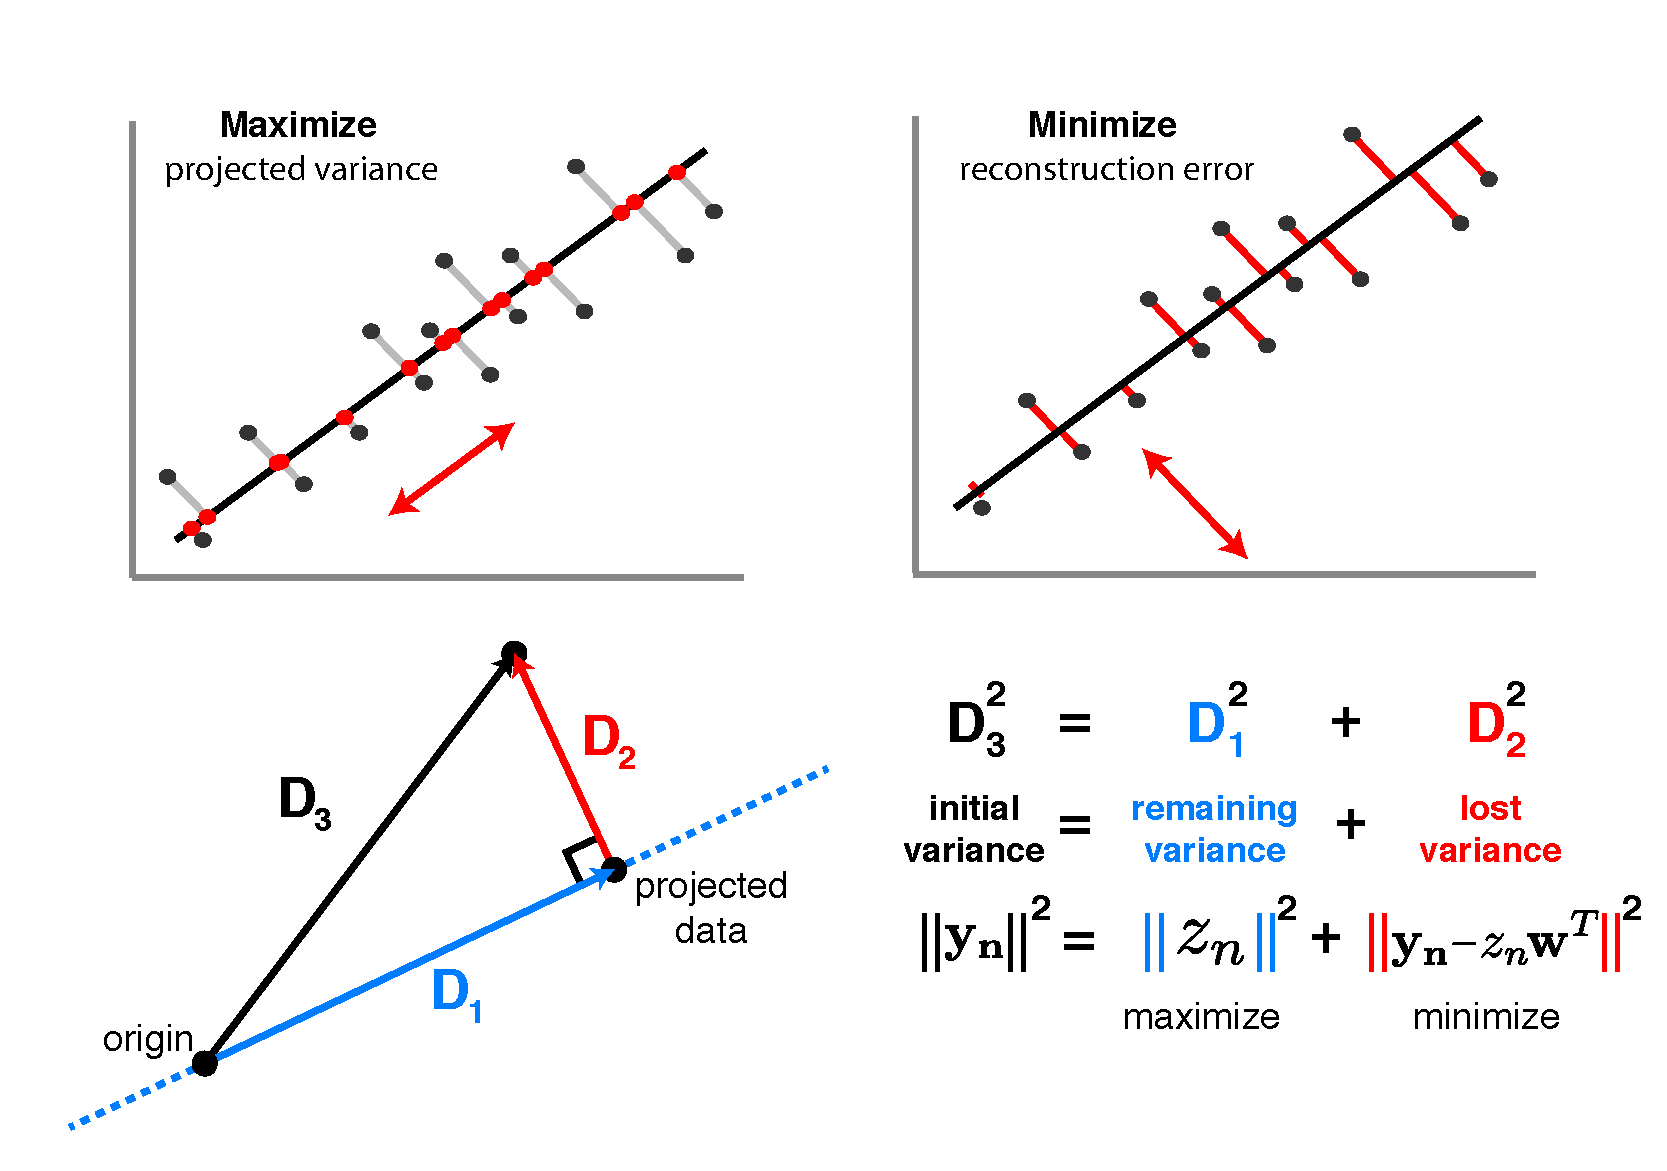
\includegraphics[width=0.8\linewidth]{pca2}
	\caption[Maximizing the variance in the principal component space is equivalent to minimizing the data reconstruction error]{In the maximum variance formulation the aim is to maximise the variance of the projected data (blue line), whereas in the minimum error formulation the aim is to minimise the residual variance (red line). Given a fixed total variance (black line), both strategies are equivalent}
	\label{fig:pca2}
\end{figure}

The main strength of PCA relies on its simplicity and closed form solution. Additionally, the linear mapping has the advantage of yielding interpretable feature weights, so that inspection of $\bfw_k$ reveals which features are jointly affected by the $k$-th principal component.\\
However, PCA suffers from serious drawbacks when applying it to real data sets \cite{Li2017b}. First, biological measurements are inherently noisy, and there is no explicit account of noise in PCA. In practice, high variance components are often asociated with signal whereas low-variance components are assumed to be noise, but an ideal model should explicitly disentangle the uncoordinated variability that is attributed to noise from the coordinated variability that is characterised as signal. Second, in its original formulation, no missing data is allowed \cite{Ilin2010}. Third, it does not offer a principled way of modelling prior information about the data.

\subsection{Probabilistic Principal Component Analysis and Factor Analysis} \label{section:probabilistic_pca}
A probabilistic version of PCA was initially proposed in \cite{Tipping1999}. It can be formulated by converting some (or all) fixed parameters into random variables and adding an explicit noise term to \Cref{eq:linear_model}:
\begin{equation}
	\bfY = \bfW \bfZ + \bepsilon
\end{equation}
where the weights $\bfW$ are assumed to be non-probabilistic parameters, but the noise $\bepsilon$ and the latent variables $\bfZ$ (the principal components) are assumed to follow an isotropic normal distribution:
\begin{align*}
	p(\bfZ) &= \prod_{n=1}^{N} \prod_{k=1}^{K} \Ndist{z_{nk}}{0,1} \\
	p(\epsilon) &= \Ndist {\epsilon}{0,\sigma^2}
\end{align*}
%The alternative strategy of treating $\bfZ$ as random variables and $\bfW$ as parameters has also been explored \cite{Lawrence2005}.\\

All together, this leads to a normally-distributed likelihood:
\begin{equation} \label{eq:ppca_lik}
	% p(\bfY|\bfW,\bfZ,\sigma) = \Ndist{\bfY}{\bfW \bfZ,\sigma^2 \I}
	p(\bfY|\bfW,\bfZ,\sigma) = \prod_{n=1}^{N} \prod_{d=1}^{D} \Ndist{y_{n,d}}{\bfw_{,:k}^T \bfz_{n,:},\sigma^2 \I}
\end{equation}

The corresponding graphical model is:

\begin{figure}[H]
	\centering
	% \definecolor{colD}{rgb}{0.2, 0.2, 0.6}
\definecolor{colM}{rgb}{0.0, 0.5, 0.0}
\definecolor{colN}{rgb}{0.5, 0.0, 0.13}
\definecolor{colG}{rgb}{1.0, 0.65, 0.0}
\newcommand\op{0.25}
\colorlet{shadecolor}{black!25}


\begin{tikzpicture}

% Define nodes
\node[obs]   (Y) {$y_{n,d}$};
\node[latent, xshift=-1.5cm, above=of Y, yshift=-0.4cm] (Z) {$z_{n,k}$};
\node[latent, double, double distance=1pt, above=of Y, yshift=0.6cm] (W) {$w_{d,k}$};
\node[latent, double, double distance=1pt, xshift=1.5cm] (Tau) {$\tau$};

% Connect the nodes
\edge {Z,W, Tau} {Y};

% Plates
\plate[] {plateK} {(Z)(W)} {$K$};
\plate[] {plateN} {(Y)(Z)(plateK.south east)(plateK.south west)} {$N$};
\plate[] {plateD} {(Y)(W)(plateK.north east)(plateN.south east)} {$D$};

\end{tikzpicture}
	\caption{Graphical model for probabilistic PCA. The latent variables are modelled as random variables, whereas the weights and the noise are modelled as deterministic parameters.}
	\label{fig:pPCA}
\end{figure}

Importantly, the choice of the distribution for $\epsilon$ implies that the noise of each feature is independent but restricted to have the same variance $\sigma^2$. In practice this is a limiting assumption, as different features are expected to show different degrees of noise, albeit this constraint can be relaxed and forms the basis of Factor Analysis \cite{Rubin1982,Bishop2006}.

The inference procedures involves learning the parameters $\bfW$, and $\sigma^2$ and a posterior probability distribution for $\bfZ$. As the model depends on latent variables, inference can be performed using the iterative Expectation-Maximisation (EM) algorithm \cite{Rubin1982,Bishop2006}. In the expectation step, the posterior distribution for $\bfZ$ is computed in closed form (due to conjugacy between the likelihood and the prior), given current estimates for the parameters $\bfW$, and $\sigma^2$. In the maximisation step, the parameters are calculated by maximising the expectation of the joint log likelihood under the posterior distribution of $\bfZ$ found in the E step \cite{Tipping1999}.\\
Interestingly, the EM solution of probabilistic PCA lies in the same subspace as the traditional PCA solution \cite{Tipping1999}, but the use of a probabilistic framework brings several benefits. First, model selection can be performed by comparing likelihoods across different settings of parameters. Second, missing data can naturally be accounted for by ignoring the missing observations from the likelihood. Finally, the probabilistic formulation sets the core framework for a Bayesian treatment of PCA, enabling a broad range of principled extensions tailored different types of data sets.


\subsection{Bayesian Principal Component Analysis and Bayesian Factor Analysis} \label{section:bayesian_pca}

The full Bayesian treatment of PCA requires the specification of prior probability distributions for all unobserved variables:
\begin{align*}
	p(\bfZ) &= \prod_{n=1}^{N} \prod_{k=1}^{K} \Ndist{z_{nk}}{0,1} \\
	p(\bfW) &= \prod_{d=1}^{D} \prod_{k=1}^{K} \Ndist{w_{dk}}{0,1} \\
	p(\epsilon) &= \Ndist {\epsilon}{0,\tau^{-1}} \\
	p(\tau) &= \Gdist{\tau}{a_0,b_0}
\end{align*}
where $\tau$ is the precision (inverse of the variance) of the noise term. A generalisation to Bayesian Factor Analysis follows by allowing a separate noise term per feature:
\begin{align*}
	p(\bepsilon) &= \prod_{d=1}^{D} \Ndist {\epsilon_d}{0,\tau_d^{-1}} \\
	p(\btau) &= \prod_{d=1}^{D} \Gdist{\tau_d}{a_0,b_0}
\end{align*}
where $a_0$ and $b_0$ are fixed hyperparameters. As in \Cref{eq:ppca_lik}, this results in a Normal likelihood:
\[
	p(\bfY|\bfW,\bfZ,\btau) = \prod_{n=1}^{N} \prod_{d=1}^{D} \Ndist{y_{nd}}{\bfw_{d}^T \bfz_{n},\tau_d}
\]

The corresponding graphical model is:

\begin{figure}[H] 
	\centering
	\begin{tikzpicture}

% Define nodes
\node[obs]   (Y) {$y_{n,d}$};
\node[latent, above=of Y, xshift=-1.5cm] (Z) {$z_{n,k}$};
\node[latent, above=of Y, xshift=1.5cm] (W) {$w_{d,k}$};
\node[latent, xshift=1.5cm] (Tau) {$\tau_{d}$};

% Connect the nodes
\edge {Z,W, Tau} {Y};

% Plates
\plate[] {plateK} {(Z)(W)} {$K$};
\plate[] {plateN} {(Y)(Z)(plateK.north west)} {$N$};
\plate[] {plateD} {(Y)(W)(Tau)(plateK.south east) (plateN.south east) (plateN.north east)} {$D$};

\end{tikzpicture}
	\caption{Graphical model for Bayesian Factor Analysis. All unobserved variables are modelled as random variables.}
	\label{fig:bayesianFA}
\end{figure}


\subsection{Hierarchical priors}  \label{section:hierarchical_priors}

A key advantage of the full Bayesian treatment is that it explicitly captures uncertainity on the estimation of all unobserved variables, as opposed to the probabilistic PCA model \cite{Bishop1999a,Bishop1999b}. Yet, more importantly, the use of (hierarchical) prior distributions allow different modelling assumptions to be encoded, providing a flexible and principled approach to extend PCA to a myriad of modelling scenarios, including multi-view generalisations \cite{Klami2008,Virtanen2012,Klami2015,Bunte2016,Khan2014,Zhao2016}.

\subsubsection{Automatic relevance determination} \label{section:ard}


As an example, a major challenge in PCA is how to determine the dimensionality of the latent space (i.e. the number of principal components). As we will show, the use of hierarchical prior distributions allows the model to introduce sparsity assumptions on the weights in such a way that the model automatically learns the number of factors.\\
In the context of Factor Analysis, one the first sparsity priors to be proposed was the Automatic Relevance determination (ARD) prior \cite{Neal1995,Mackay1996,Bishop1999a,Bishop1999b}. 
\begin{equation*} \label{eq:ard}
	p(\bfW|\balpha) = \prod_{k=1}^{K} \Ndist{\bfw_{:,k}}{0,\frac{1}{\alpha_{k}}\I_{D}} \\
	\qquad\qquad
	p(\balpha) = \prod_{k=1}^{K} \Gdist{\alpha_k}{a_0^\alpha, b_0^\alpha}
\end{equation*}
The aim of this prior is two-fold. First, the zero-mean normal distribution specifies that, \textit{a priori}, no information is available and all features are \textit{inactive}. When exposed to some data, the posterior distribution for $\bfW$ will be estimated by weighting the contribution from the likelihood, potentially allowing features to escape from the zero-centered prior (\Cref{fig:ard}).\\
Second, performing inference on the variable $\balpha = \{ \alpha_1, \cdots, \alpha_k \}$ enables the model to discard inactive factors. To understand this, let us assume that only $K=5$ true factors exist, but the model is initialised with $K=20$ factors. In such case, inactive factors can be prunned out by driving the corresponding $\alpha_k$ to infinity. In turn, this causes the posterior $p(\bfw_{:,k}|\bfY)$ to be sharply peaked at zero, resulting in the inactivation of all its weights. %\Cref{fig:hinton}.

\begin{figure}[H] \begin{center}
	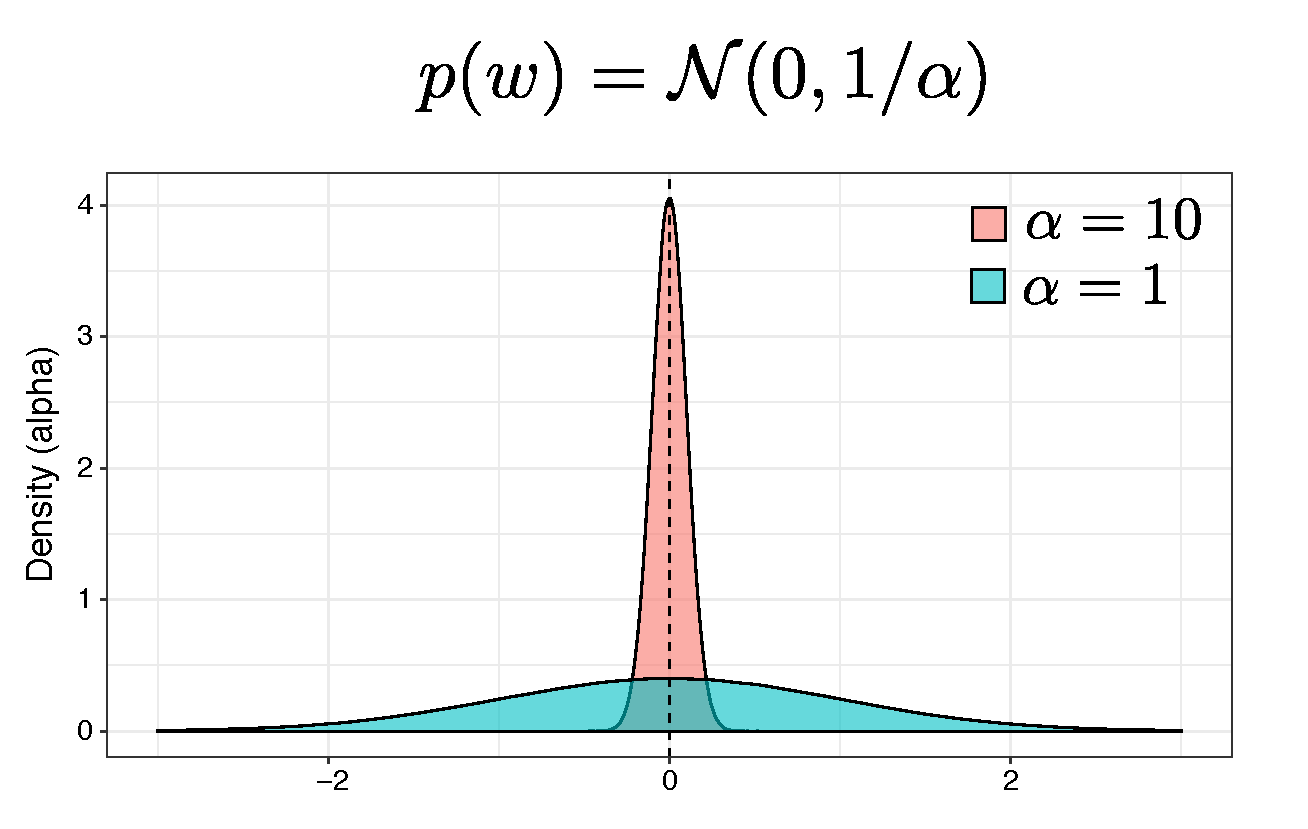
\includegraphics[width=0.7\textwidth]{Chapter2/Figs/ard}
	\caption{Visualisation of the sparsity-inducing Automatic Relevance Determination prior}
	\label{fig:ard}
\end{center} \end{figure}

% \begin{figure}[H] \begin{center}
% 	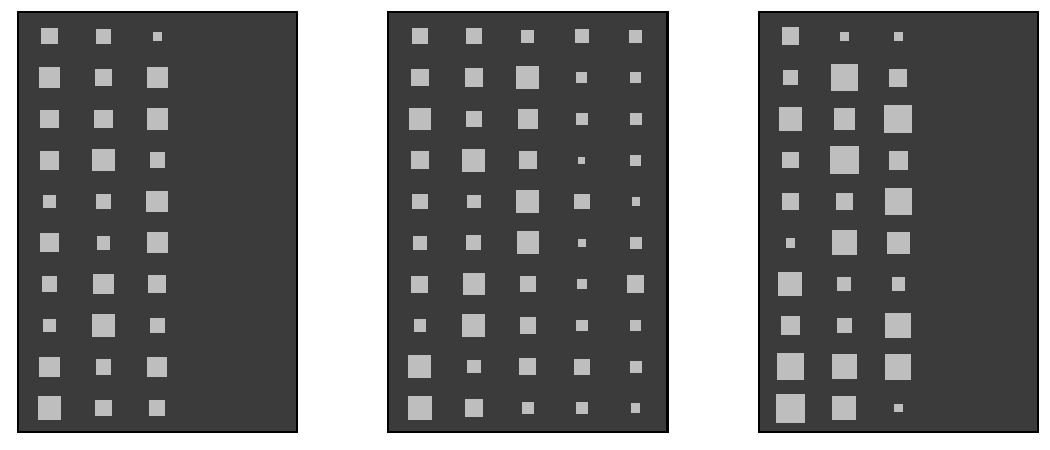
\includegraphics[width=0.8\textwidth]{Chapter2/Figs/hinton}
%             \caption[Hinton plot of the weight matrix for a Bayesian Factor Analysis model with an ARD prior]{Hinton plots display the values of the weight matrix, similar to a heatmap, where bigger squares depict larger weights. Shown are the Hinton plots for (a) the true weights, (b) the infered weights by a Factor Analysis model with no ARD prior (middle), and (c) the infered weights by a Factor Analysis model with ARD prior per factor. This figure was generated using simulated data with $N=100$ samples, $D=10$ features and $K=3$ factors.}
% 	\label{fig:hinton}
% \end{center} \end{figure}

\subsubsection{Spike-and-slab prior} \label{section_spikeslab}

Sparse extensions of the Bayesian factor analysis model have been proposed as a regularisation mechanism but also to model inherent assumptions regarding the sparse nature of biological data \cite{Stegle2012,Gao2013}.\\
The variability observed in biological data is driven both by technical factors and biological factors. Technical factors (i.e. batch effects) tend to be relatively strong and alter the expression of a large proportion of genes, whereas the biological factors are potentially weak effects driven by changes in small gene regulatory networks \cite{Gao2013}. Hence, a practical factor analysis model should be able to learn factors with different degrees of sparsity.\\
The ARD prior proposed in \Cref{eq:ard} allows entire factors to be dropped out from the model, but it provides a weak degree of regularisation when it comes to inactivating individual weights within the active factors.

A sparse generalisation of the Factor Analysis model proposed above can be achieved by combining the ARD prior with a spike-and-slab prior \cite{Mitchell1988,Titsias2011}:
\begin{align}
	p(w_{d,k} \mid \alpha_k,\theta_k) &= (1-\theta_k) \mathds{1}_0(w_{d,k}) + \theta_k \Ndist{w_{d,k}}{0, \alpha_k^{-1}} \\
	p(\theta_k) &= \Bdist{\theta_k}{a_0^\theta,b_0^\theta} \\
	p(\alpha_k) &= \Gdist{\alpha_k}{a_0^\alpha, b_0^\alpha}
\end{align}

The corresponding graphical model is:

\begin{figure}[H] \begin{center}
	\begin{tikzpicture}

% Define nodes
\node[obs]   (Y) {$y_{n,d}$};
\node[latent, above=of Y, xshift=-1.5cm] (Z) {$z_{n,k}$};
\node[latent, above=of W, xshift=-0.75cm] (Theta) {$\theta_{k}$};
\node[latent, above=of W, xshift=0.75cm] (Alpha) {$\alpha_{k}$};
\node[latent, above=of Y, xshift=1.5cm] (W) {$w_{d,k}$};
\node[latent, xshift=1.5cm] (Tau) {$\tau_{d}$};

% Connect the nodes
\edge {Theta, Alpha} {W};
\edge {Z, W, Tau} {Y};

% Plates
\plate[] {plateK} {(Z)(W)(Theta)(Alpha)} {$K$};
% \plate[] {plateN} {(Y)(Z)(plateK.north west)} {$N$};
\plate[] {plateN} {(Y)(Z)} {$N$};
\plate[] {plateD} {(Y)(W)(Tau)(plateK.south east) (plateN.south east) (plateN.north east)} {$D$};

\end{tikzpicture}
	\label{fig:bayesianFA}
	\caption{Graphical model for Bayesian sparse Factor Analysis. A double sparsity-inducing prior is used on the weights: an ARD prior to prune inactive factors and a spike-and-slab prior to inactive individual features within the active factors.}
\end{center} \end{figure}

The spike-and-slab prior is effectively a mixture model where features are sampled from a zero-inflated Gaussian distribution, where $\theta_k \in (0,1)$ dictates the level of sparsity per factor (i.e. how many active features). A value of $\theta_k$ close to $0$ implies that most of the weights of factor $k$ are shrunk to $0$ (i.e. a sparse factor), whereas a value of $\theta_k$ close to $1$ implies that most of the weights are non-zero (i.e. dense factors). By learning $\theta_k$ from the data, the model naturally accounts for combinations of sparse and dense factors.


% \subsubsection{Inference}
% In a fully Bayesian setting, the inference procedure corresponds to learning the posterior distributions for each unobserved variable. However, applying Bayes rule yields an analytically intractable solution, and approximate methods are required. This is discussed in Chapter X.



\subsection{Multi-view factor analysis models}

Probabilistic PCA and Factor Analysis perform dimensionality reduction from a single input matrix. In some occasions data is collected from multiple data sources that exibit heterogeneous statistical properties, resulting in a structured data set where features are naturally partitioned into views \cite{Xu2013,Li2016,Zeng2018}. A clear biological example is multi-omics data, where, for the same set of samples, multiple molecular layers are profiled. Each of the data modalities can be analysed separately using conventional (single-view) methods, but in the ideal strategy a single model should be used to leverage information across all molecular layers using a flexible and principled approach. This is referred to as the multi-view learning problem \cite{Xu2013,Li2016}.\\
A tempting approach to circumvent the multi-view learning problem is to simply concatenate all data sets before applying conventional (single-view) latent variable models \cite{Ritchie2015}. However, this is prone to fail for several reasons. First, heterogeneous data modalities cannot always be modelled using the same likelihood function. For example, continuous measurements are often modelled using a normal distribution, but binary and count-based traits are not appropriately modelled by this distribution \cite{Pilling2018}. Second, even if all views are modelled with the same likelihood, differences in the scale and the magnitude of the variance can lead to some views being overrepresented in the latent space. Finally, in a multi-view data set we expect multiple sources of variation, some driven by a single view, whereas others could capture shared variability across multiple views. In other words, from a structured input space, one can also expect a structured latent representation. Not taking this behaviour into account can lead to challenges in the interpretability of the latent space.

A comprehensive review of multi-view machine learning methods can be found in \cite{Xu2013} and a more genomics-oriented perspective in \cite{Ritchie2015}. For the purpose of this thesis, I will describe only the use of latent variable models for multi-view data integration.

\subsection{Canonical Correlation Analysis} \label{cca}

Canonical Correlation Analysis (CCA) is a simple extension of PCA to find linear components that capture correlations between two datasets \cite{Hotteling1936,Hardle2007}.\\
Given two data matrices $\bfY_1 \in \R^{N \times D_1}$ and $\bfY_2 \in \R^{N \times D_2}$ CCA finds a set of linear combinations $\bfU \in \R^{D_1 \times K}$ and $\bfV \in \R^{D_2 \times K}$ with maximal cross-correlation.
For the first pair of canonical variables, the optimisation problem is:
\[
	(\hat{\bfu_1}, \hat{\bfv_1}) = \argmax_{\bfu_1,\bfv_1} corr(\bfu_{1}^T \bfY_1, \bfv_{1}^T \bfY_2)
\]
As in conventional PCA, the linear components are constraint to be orthogonal. Hence, the first pair of canonical variables $\bfu_1$ and $\bfv_1$ contain the linear combination of variables that have maximal correlation. Subsequently, the second pair of canonical variables $\bfu_2$ and $\bfv_2$ is found from the residuals of the first canonical variables.

Given the similarity with PCA, both methods share statistical properties, including the linear mapping between the low-dimensional space and the high-dimensional space, and the closed-form solution using singular value decomposition \cite{Hotteling1936,Hardle2007}.\\
Because of its simplicity and efficient computation, CCA has widespread use as a dimensionality reduction technique \cite{Hardle2007}. Yet, as expected, CCA suffers from the same pitfalls as PCA: difficulties in selecting the number of components, lack of sparsity in the solutions and absence of probabilistic formulation. In addition, CCA have been shown to overfit for datasets where $D>>N$ \cite{McCabe2018,Guo2016}. Hence, probabilistic versions with sparsity assumptions that reduce overfitting and improve interpretability followed.


\subsubsection{Probabilistic Canonical Correlation Analysis} \label{section_probabilisticCCA}

Following the derivation of probabilistic PCA \cite{Tipping1999}, a similar effort enabled a probabilistic formulation of CCA as a generative model \cite{Bach2005}.\\
In this model, the two matrix of observations $\bfY^{1}$ and $\bfY^{2}$ are decomposed in terms of two weight matrices $\bfW^{1}$ and $\bfW^{2}$ but a joint latent matrix $\bfZ$:
\begin{align*}
	\bfY^{1} &= \bfW^{1} \bfZ + \epsilon^{1} \\
	\bfY^{2} &= \bfW^{2} \bfZ + \epsilon^{2}
\end{align*}
With the following prior probability distributions:
\begin{align*}
	p(z_{nk}) &= \Ndist{z_{nk}}{0,1} \\
	p(\epsilon^{1}) &= \Ndist {\epsilon^{1}}{\tau_{1}^{-1}} \\
	p(\epsilon^{2}) &= \Ndist {\epsilon^{2}}{\tau_{2}^{-1}}
\end{align*}
As in \cite{Tipping1999}, the weights and the variance of the noise are assumed to be non-probabilistic parameters, whereas the factors are probabilistic unobserved variables. This yields the following likelihood functions:
\begin{align} \label{eq:probabilistic_cca_likelihood}
	p(\bfY^{1}|\bfW^{1},\bfZ,\tau_{1}) &= \prod_{n=1}^{N} \prod_{d=1}^{D_1} \Ndist{y^{1}_{n,d}}{(\bfw_{:,k}^{1})^T \bfz_{n},\tau_{1}^{-1}} \\
	p(\bfY^{2}|\bfW^{2},\bfZ,\tau_{2}) &= \prod_{n=1}^{N} \prod_{d=1}^{D_2} \Ndist{y^{2}_{n,d}}{(\bfw_{:,k}^{2})^T \bfz_{n},\tau_{2}^{-1}} \nonumber
\end{align}

The corresponding graphical model is:
\begin{figure}[H] \begin{center}
	\begin{tikzpicture}

% Define nodes
\node[obs, xshift=-1.5cm] (Y1) {$y^{1}_{n,d}$};
\node[obs, xshift=+1.5cm] (Y2) {$y^{2}_{n,d}$};

\node[latent, below=of Y1, yshift=+0.5cm, xshift=+1.5cm] (Z) {$z_{n,k}$};

\node[latent, double, double distance=1pt, below=of Y1, xshift=-1cm, yshift=-1cm] (W1) {$w^{1}_{d,k}$};
\node[latent, double, double distance=1pt, below=of Y2, xshift=+1cm, yshift=-1cm] (W2) {$w^{2}_{d,k}$};

\node[latent, double, double distance=1pt, left=of Y1, yshift=-0.5cm] (Tau1) {$\tau^{1}$};
\node[latent, double, double distance=1pt, right=of Y2, yshift=-0.5cm] (Tau2) {$\tau^{2}$};

% Connect the nodes
\edge {Z} {Y1};
\edge {Z} {Y2};
\edge {W1} {Y1};
\edge {W2} {Y2};
\edge {Tau1} {Y1};
\edge {Tau2} {Y2};
% \edge {Z,W, Tau} {Y};

% Plates
\plate[] {plateK} {(Z)(W1)(W2)} {$K$};
% \plate[] {plateN} {(Y1)(Y2)(Z)(plateD1.north)} {$N$};
% \plate[] {plateD1} {(Y1)(W1)(plateK.south)(plateN.north)} {$D_1$};
% \plate[] {plateD2} {(Y2)(W2)(plateK.south)(plateN.north)} {$D_2$};
\plate[] {plateN} {(Y1)(Y2)(Z)} {$N$};
\plate[] {plateD1} {(Y1)(W1)(Tau1)} {$D_1$};
\plate[] {plateD2} {(Y2)(W2)(Tau2)} {$D_2$};

\end{tikzpicture}



	\label{fig:graphical_CCA}
	\caption{Graphical model for probabilistic Canonical Correlation Analysis}
\end{center} \end{figure}

Notice that the observations for both data sets are generated from the same set of latent variables $\bfZ$. This ensures that the model is focused on capturing the variation associated with cross-correlated groups of features.

Analogously to probabilistic PCA, the expected value of the posterior distribution $p(\bfZ|\bfY^{1},\bfY^{2})$ span the same subspace as standard CCA \cite{Bach2005}. Nonetheless, one of the many advantage of a probabilistic formulation is that it enables a broad range of principled extensions into larger graphical models.


\subsubsection{Bayesian Canonical Correlation Analysis} \label{section:bayesian_cca}

A fully Bayesian treatment of CCA followed based on exactly the same principle presented in \Cref{section:bayesian_pca} by introducing prior distributions to all unobserved variables \cite{Wang2007,Klami2013}:
\begin{align*} 
	p(\bfZ) &= \prod_{n=1}^{N} \prod_{k=1}^{K} \Ndist{z_{nk}}{0,1} \\
	p(\epsilon^{1}) &= \Ndist {\epsilon^{1}}{\sigma_{1}^{2}} \\
	p(\epsilon^{2}) &= \Ndist {\epsilon^{2}}{\sigma_{2}^{2}} \\
	p(\bfW^1|\balpha) &= \prod_{k=1}^{K} \Ndist{\bfw^{1}_{:,k}}{0,\frac{1}{\alpha_{k}}\I_{D_1}} \\
	p(\bfW^2|\balpha) &= \prod_{k=1}^{K} \Ndist{\bfw^{2}_{:,k}}{0,\frac{1}{\alpha_{k}}\I_{D_2}} \\
	p(\balpha) &= \prod_{k=1}^{K} \Gdist{\alpha_k}{a_0^\alpha, b_0^\alpha}
\end{align*}
Resulting in the same likelihood model as in \Cref{eq:probabilistic_cca_likelihood}. Yet, notice that an ARD is introduced per factor, allowing an automatic inference of the dimensionality in the latent subspace.
Also, there is some flexibility in the definition of noise. Whereas an independent noise term can be defined per view, one can also model correlated noise by introducing a multivariate Gaussian distribution with full-rank covariance \cite{Wang2007,Klami2013}.

The corresponding graphical model is:
\begin{figure}[H] \begin{center}
	\begin{tikzpicture}

% Define nodes
\node[obs, xshift=-1.5cm] (Y1) {$y^{1}_{n,d}$};
\node[obs, xshift=+1.5cm] (Y2) {$y^{2}_{n,d}$};

\node[latent, below=of Y1, yshift=+0.5cm, xshift=+1.5cm] (Z) {$z_{n,k}$};

\node[latent, below=of Y1, xshift=-1cm, yshift=-1cm] (W1) {$w^{1}_{d,k}$};
\node[latent, below=of Y2, xshift=+1cm, yshift=-1cm] (W2) {$w^{2}_{d,k}$};

\node[latent, left=of Y1, yshift=-0.5cm] (Tau1) {$\tau^{1}$};
\node[latent, right=of Y2, yshift=-0.5cm] (Tau2) {$\tau^{2}$};

% Connect the nodes
\edge {Z} {Y1};
\edge {Z} {Y2};
\edge {W1} {Y1};
\edge {W2} {Y2};
\edge {Tau1} {Y1};
\edge {Tau2} {Y2};
% \edge {Z,W, Tau} {Y};

% Plates
\plate[] {plateK} {(Z)(W1)(W2)} {$K$};
% \plate[] {plateN} {(Y1)(Y2)(Z)(plateD1.north)} {$N$};
% \plate[] {plateD1} {(Y1)(W1)(plateK.south)(plateN.north)} {$D_1$};
% \plate[] {plateD2} {(Y2)(W2)(plateK.south)(plateN.north)} {$D_2$};
\plate[] {plateN} {(Y1)(Y2)(Z)} {$N$};
\plate[] {plateD1} {(Y1)(W1)(Tau1)} {$D_1$};
\plate[] {plateD2} {(Y2)(W2)(Tau2)} {$D_2$};

\end{tikzpicture}
	\label{fig:graphical_bayesianCCA}
	\caption{Graphical model for Bayesian Canonical Correlation Analysis}
\end{center} \end{figure}

As expected, the sparsity priors yield a more sparse solution than traditional CCA, which is more appropriate for biological data analysis. However, this solution is still limited to $M=2$ views, which leads us to the next model extension.

% (\Cref{fig:hinton_cca}):
% \begin{figure}[H]
% 	\centering
% 	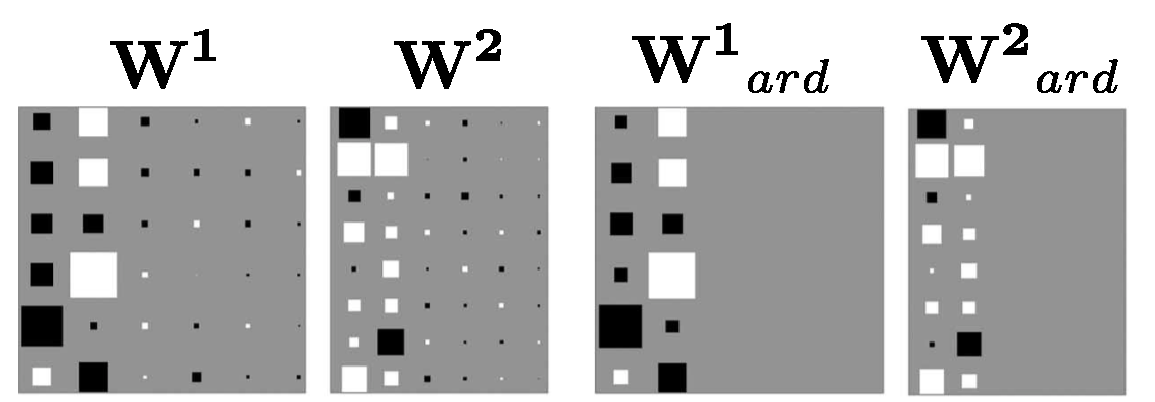
\includegraphics[width=0.85\linewidth]{hinton_cca}
% 	\caption{Comparison of the Hinton's diagram of $\bfW^{1}$ and $\bfW^{2}$ for the maximum likelihood CCA model (two left plots) and the variational Bayes CCA model (two right plots). Reprinted from \cite{Wang2007} with modifications.}
% 	\label{fig:hinton_cca}
% \end{figure}


\subsection{Group Factor Analysis} \label{section:gfa}

Group Factor Analysis (GFA) is the natural generalisation of Bayesian Canonical Correlation Analysis to an arbitrary number of views.
The original idea was originally presented in \cite{Virtanen2012} and a series of generalisations followed, tailored with specific assumptions for different applications \cite{Klami2015,Leppaaho2017,Bunte2016,Khan2014,Zhao2016,Remes2015}. In this section we will outline the core principle of GFA.

Given a data set of $M$ views $\bfY_1, \cdots, \bfY_M$, the task of GFA is to find $K$ factors that capture the variability \textit{within} as well as the variability \textit{between} views. In other words, we want to capture factors that not only explain variance that is shared across all views but we also want to capture factors that explain variance within a single view or between different subsets of views.\\
The starting point is to generalise the Bayesian CCA model (\Cref{section:bayesian_cca}) to $M$ views:
\begin{align*}
	\bfY^{1} &= \bfW^{2} \bfZ + \epsilon^{1} \\
	\bfY^{2} &= \bfW^{2} \bfZ + \epsilon^{2} \\
	& \cdots \\
	\bfY^{M} &= \bfW^{M} \bfZ + \epsilon^{M}
\end{align*}
Notice that there is a common factor space for all views, but there is a view-specific weight matrix. The key to disentangle the activity of each factor in each view lies on the sparsity structure imposed in the weights. Intuitively, if a factor $k$ is not driving any variation in a specific view $m$ we want all the individual weights to be pushed to zero. As shown before, this behaviour can be achieved using Automatic Relevance Determination (ARD) priors. However, if we were to use the same approach as in Bayesian CCA, where the ARD prior for factor $k$ is shared across all views, then factors would be restricted to have the same activity across all views.\\
In GFA this is generalised as follows:
\begin{align}
	p(\bfW) &= \prod_{m=1}^{M} \prod_{k=1}^{K} \Ndist{\bfw_{:,k}^m}{0,\frac{1}{\alpha_k^m}} \\
	p(\balpha) &= \prod_{m=1}^{M} \prod_{k=1}^{K} \Gdist{\alpha_k^m}{a_0^\alpha, b_0^\alpha}
\end{align}
This is effectively setting an ARD prior per factor $k$ and view $m$. The matrix $\balpha \in \R^{M \times K}$ defines four types of factors: (1) Inactive factors that do not explain variance in any view, which corresponds to all values $\balpha_k$ being large. (2) Fully shared factors that explain variance across all views, which corresponds to all values $\balpha_k$ being small. (3) Unique factors that explain variance in a single view, which corresponds to all values $\balpha_k$ being large, except for one entry. (4) Partially shared factors that explain variance in a subsets views, which corresponds to a mixture of small and large values for $\balpha_k$.\\

The corresponding graphical model is:

\begin{figure}[H] \begin{center}
	% \begin{tikzpicture}

% % Define nodes
% \node[obs, xshift=-1.5cm] (Y1) {$y^{m}_{n,d}$};

% \node[latent, below=of Y1, yshift=+0.5cm, xshift=+1.5cm] (Z) {$z_{n,k}$};

% \node[latent, double, double distance=1pt, below=of Y1, xshift=-1cm, yshift=-1cm] (W1) {$w^{1}_{d,k}$};
% \node[latent, double, double distance=1pt, below=of Y2, xshift=+1cm, yshift=-1cm] (W2) {$w^{2}_{d,k}$};

% \node[latent, double, double distance=1pt, left=of Y1, yshift=-0.5cm] (Tau1) {$\tau^{1}$};
% \node[latent, double, double distance=1pt, right=of Y2, yshift=-0.5cm] (Tau2) {$\tau^{2}$};

% % Connect the nodes
% \edge {Z} {Y1};
% \edge {Z} {Y2};
% \edge {W1} {Y1};
% \edge {W2} {Y2};
% \edge {Tau1} {Y1};
% \edge {Tau2} {Y2};
% % \edge {Z,W, Tau} {Y};

% % Plates
% \plate[] {plateK} {(Z)(W1)(W2)} {$K$};
% % \plate[] {plateN} {(Y1)(Y2)(Z)(plateD1.north)} {$N$};
% % \plate[] {plateD1} {(Y1)(W1)(plateK.south)(plateN.north)} {$D_1$};
% % \plate[] {plateD2} {(Y2)(W2)(plateK.south)(plateN.north)} {$D_2$};
% \plate[] {plateN} {(Y1)(Y2)(Z)} {$N$};
% \plate[] {plateD1} {(Y1)(W1)(Tau1)} {$D_1$};
% \plate[] {plateD2} {(Y2)(W2)(Tau2)} {$D_2$};

% \end{tikzpicture}



\begin{tikzpicture}
  % Define nodes:
  % matrix factorisation level
  \node[obs]   (Y) {$y_{n,d}^m$};
  \node[latent, above=of Y, xshift=-1.5cm] (Z) {$z_{n,k}$};
  \node[latent, above=of Y, xshift=1.5cm] (W) {$w^m_{k,d}$};
  % \node[latent, xshift=1.5cm] (Tau) {$\tau^m_{d}$};
  \node[latent, xshift=2.5cm] (Tau) {$\tau^m$};
  \node[latent, above=of W] (alpha) {$\alpha^m_{k}$};

  % Connect the nodes
  \edge {Z,W,Tau} {Y}; %
  \edge {alpha} {W};

  % Plates
  \plate[] {plateK} {(Z)(W)(alpha)} {$K$};
  \plate[] {plateN} {(Y)(Z) (plateK.south west)} {$N$};
  % \plate[] {plateD} {(Y)(W) (plateK.south east) (plateN.south east) (plateN.north east)} {$D_m$};
  \plate[] {plateD} {(Y)(W)} {$D_m$};
  % \plate[] {plateM} {(Tau) (plateK.north east)(plateD.south east)(plateD.south west)} {$M$};
  \plate[] {plateM} {(Y)(W)(Tau)(alpha)} {$M$};
\end{tikzpicture}

	\label{fig:graphical_GFA}
	\caption{Graphical model for Bayesian Group Factor Analysis}
\end{center} \end{figure}


Finally, notice that if $M=1$ the model reduces to Bayesian PCA (\Cref{section:bayesian_pca}), but when $M=2$ the model does \textit{not} reduce to Bayesian CCA because in the GFA setting factors are also allowed to capture both inter-specific variability (i.e. across views) and intra-specific variability (within a view). In Bayesian CCA, the views share a common ARD prior per factor to enforce the factors to explain variation in both views, at the expense of ignoring sources of variability that are specific to a single view.
